\begin{figure*}[htbp]
	\centering
	\textbf{Proprietary}\\[0.2cm]
	\begin{subfigure}[t]{0.49\linewidth}
		\centering
		\textbf{Bugs}\\[0.1cm]
		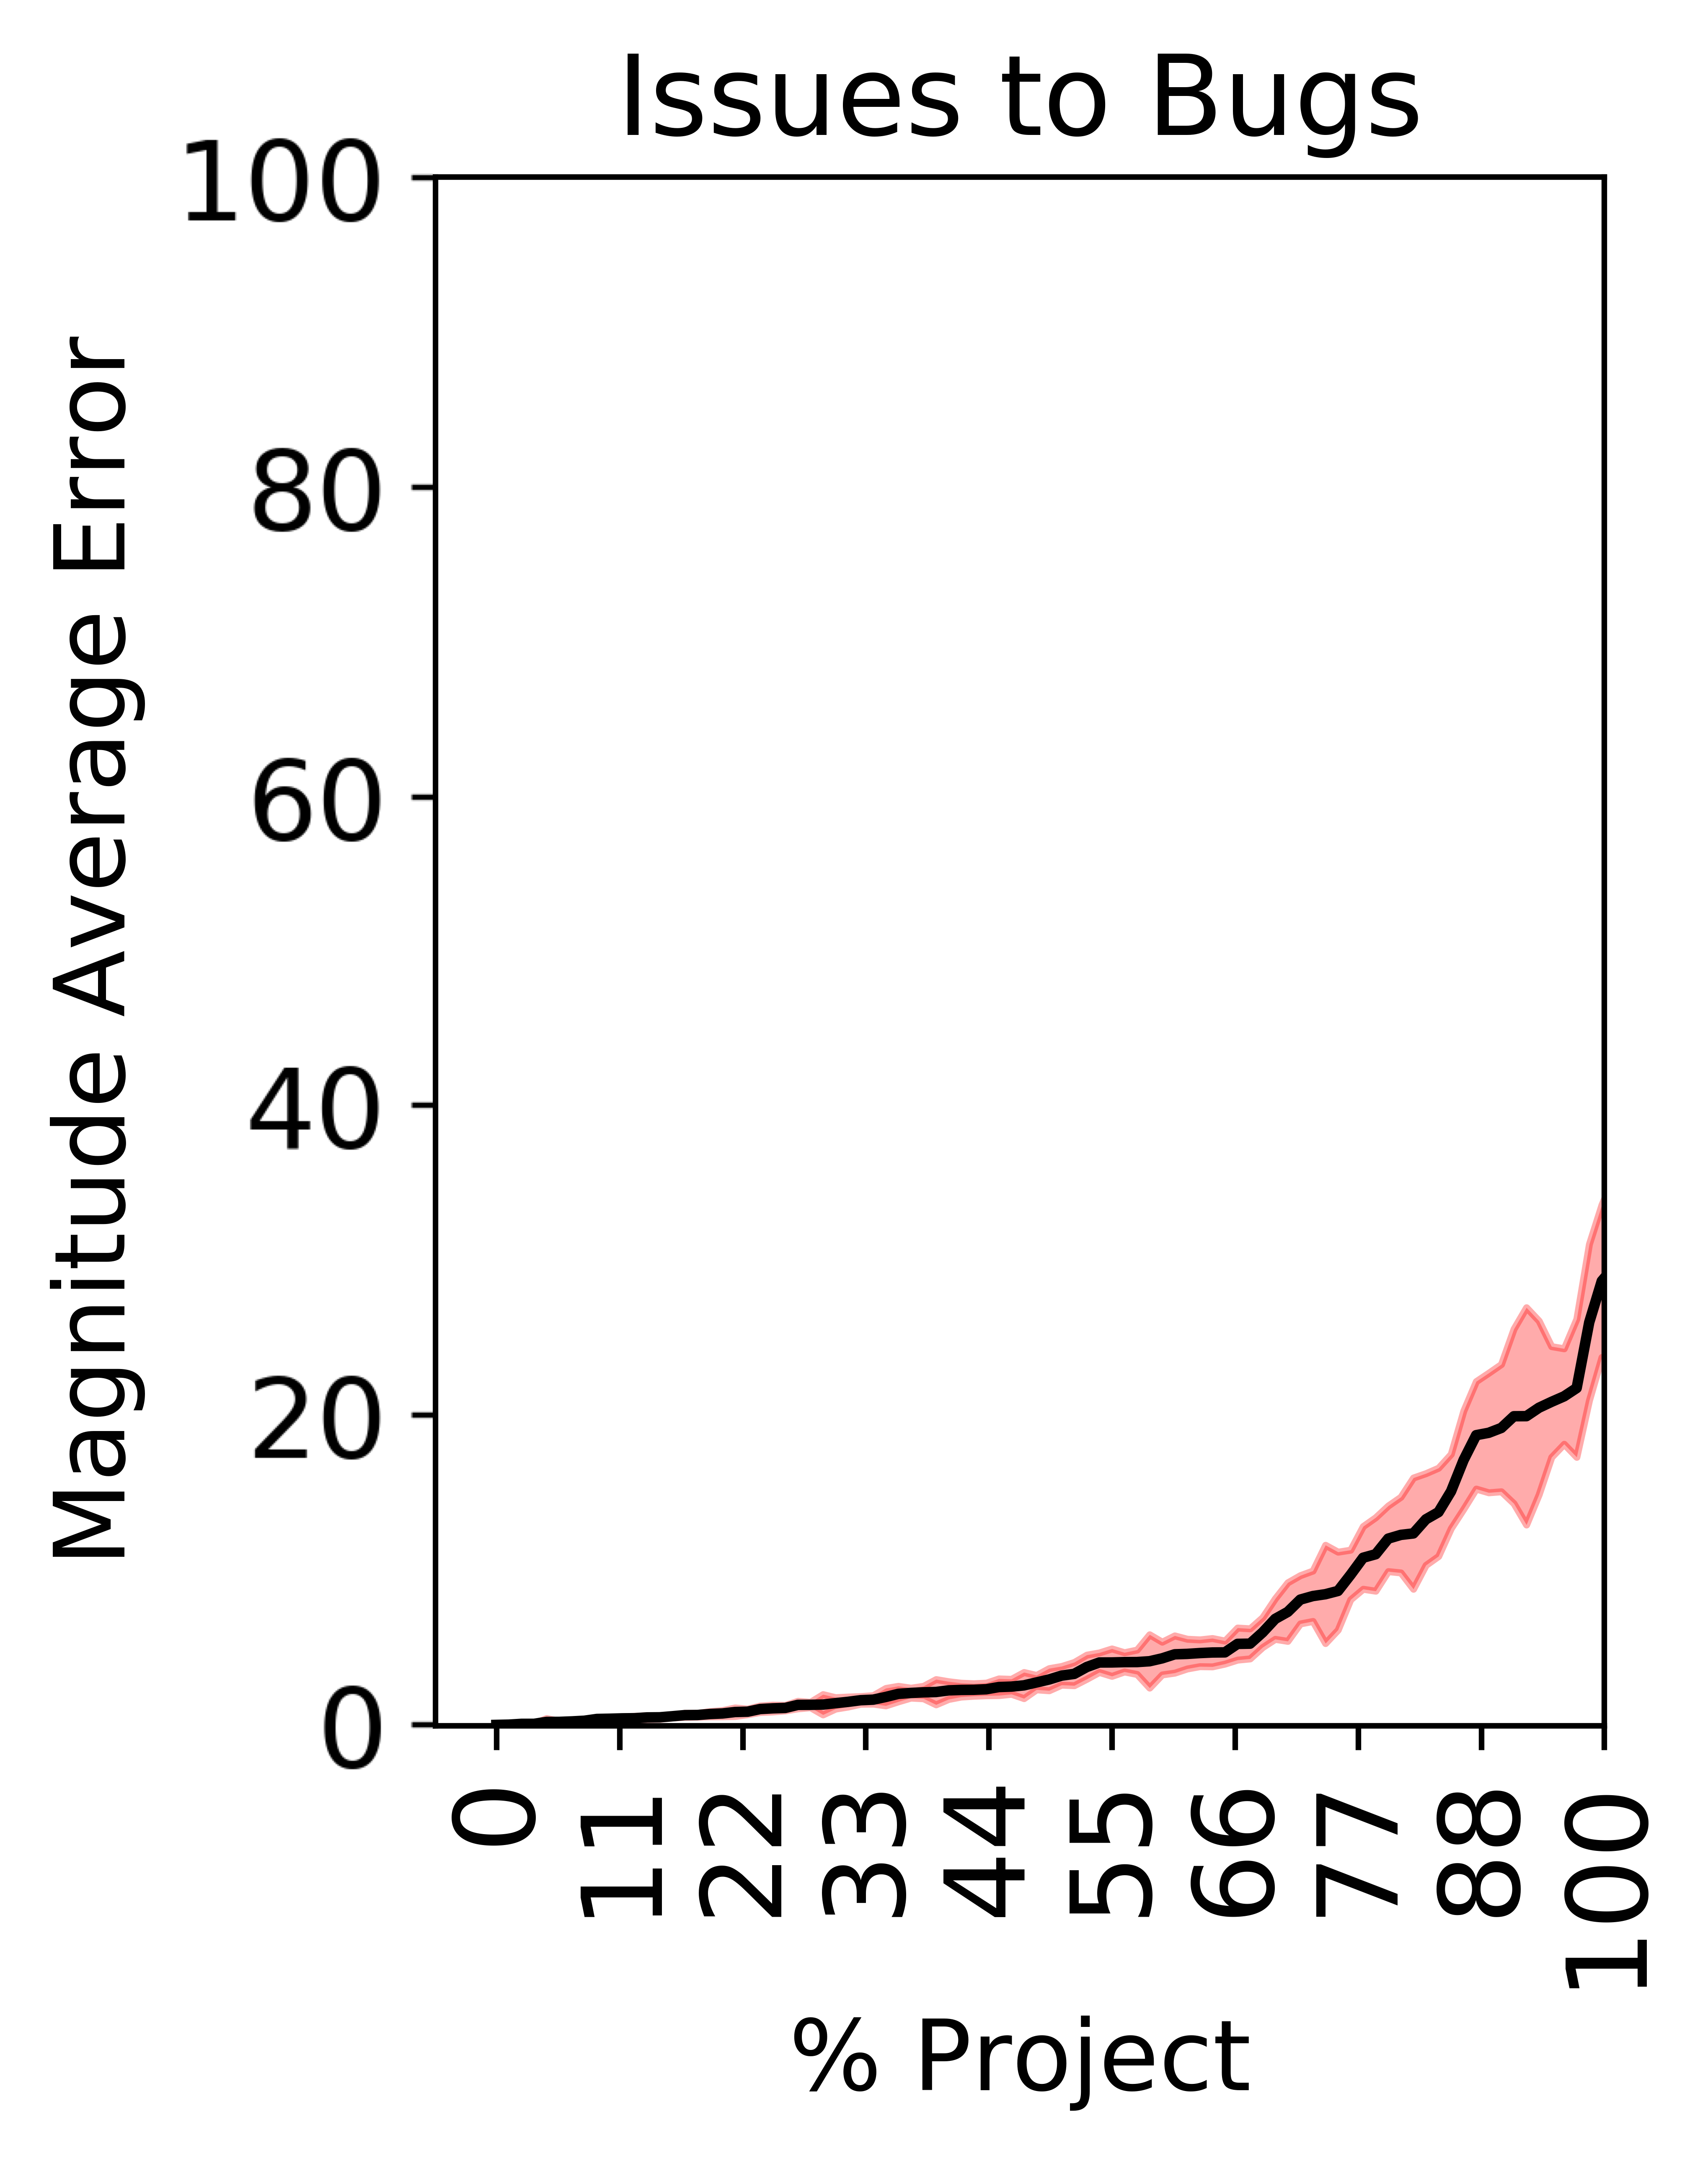
\includegraphics[width=0.335\linewidth]{images/RQ3/inhouse/bugs/1.png}
		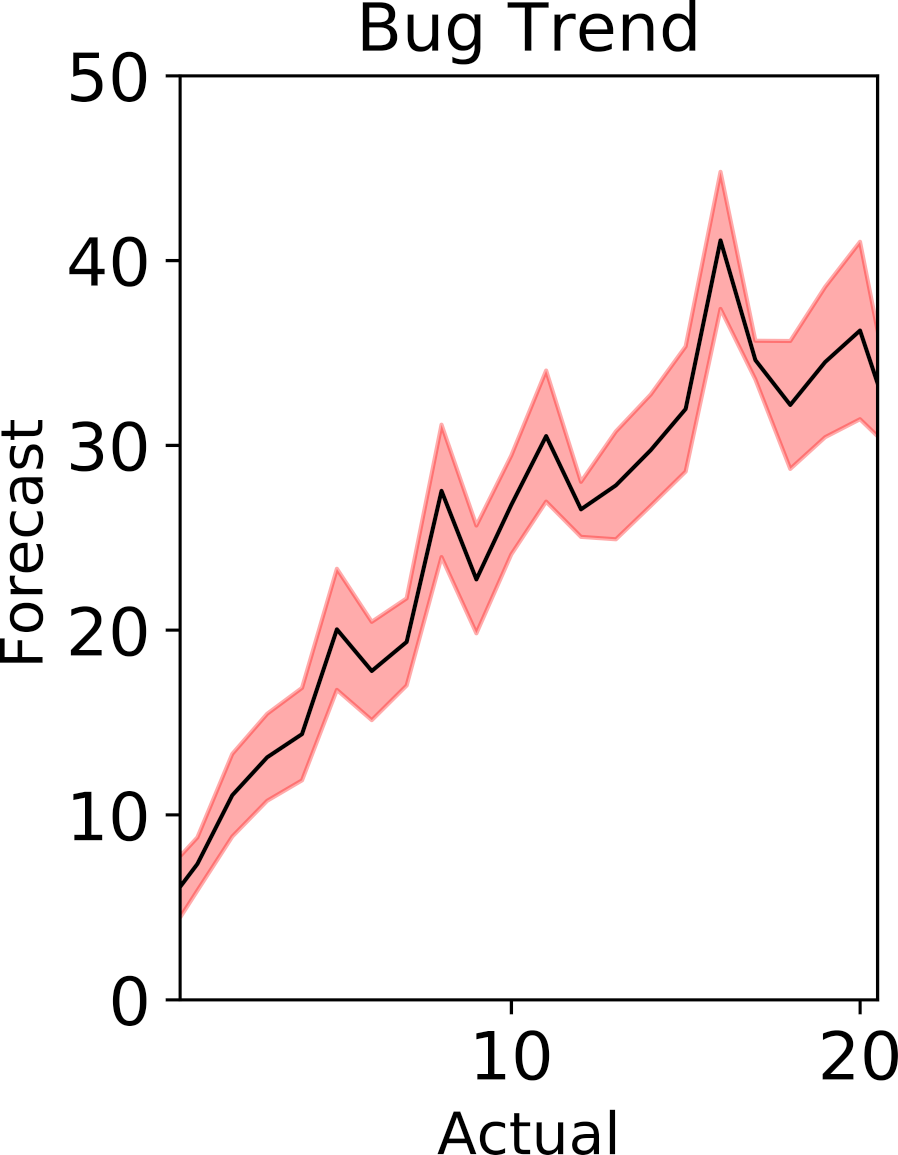
\includegraphics[width=0.33\linewidth]{images/RQ3/inhouse/bugs/2.png}
\end{subfigure}%
	%
	\centering
		\begin{subfigure}[t]{0.5\linewidth}
		\centering
		\textbf{Enhancements}\\[0.1cm]
		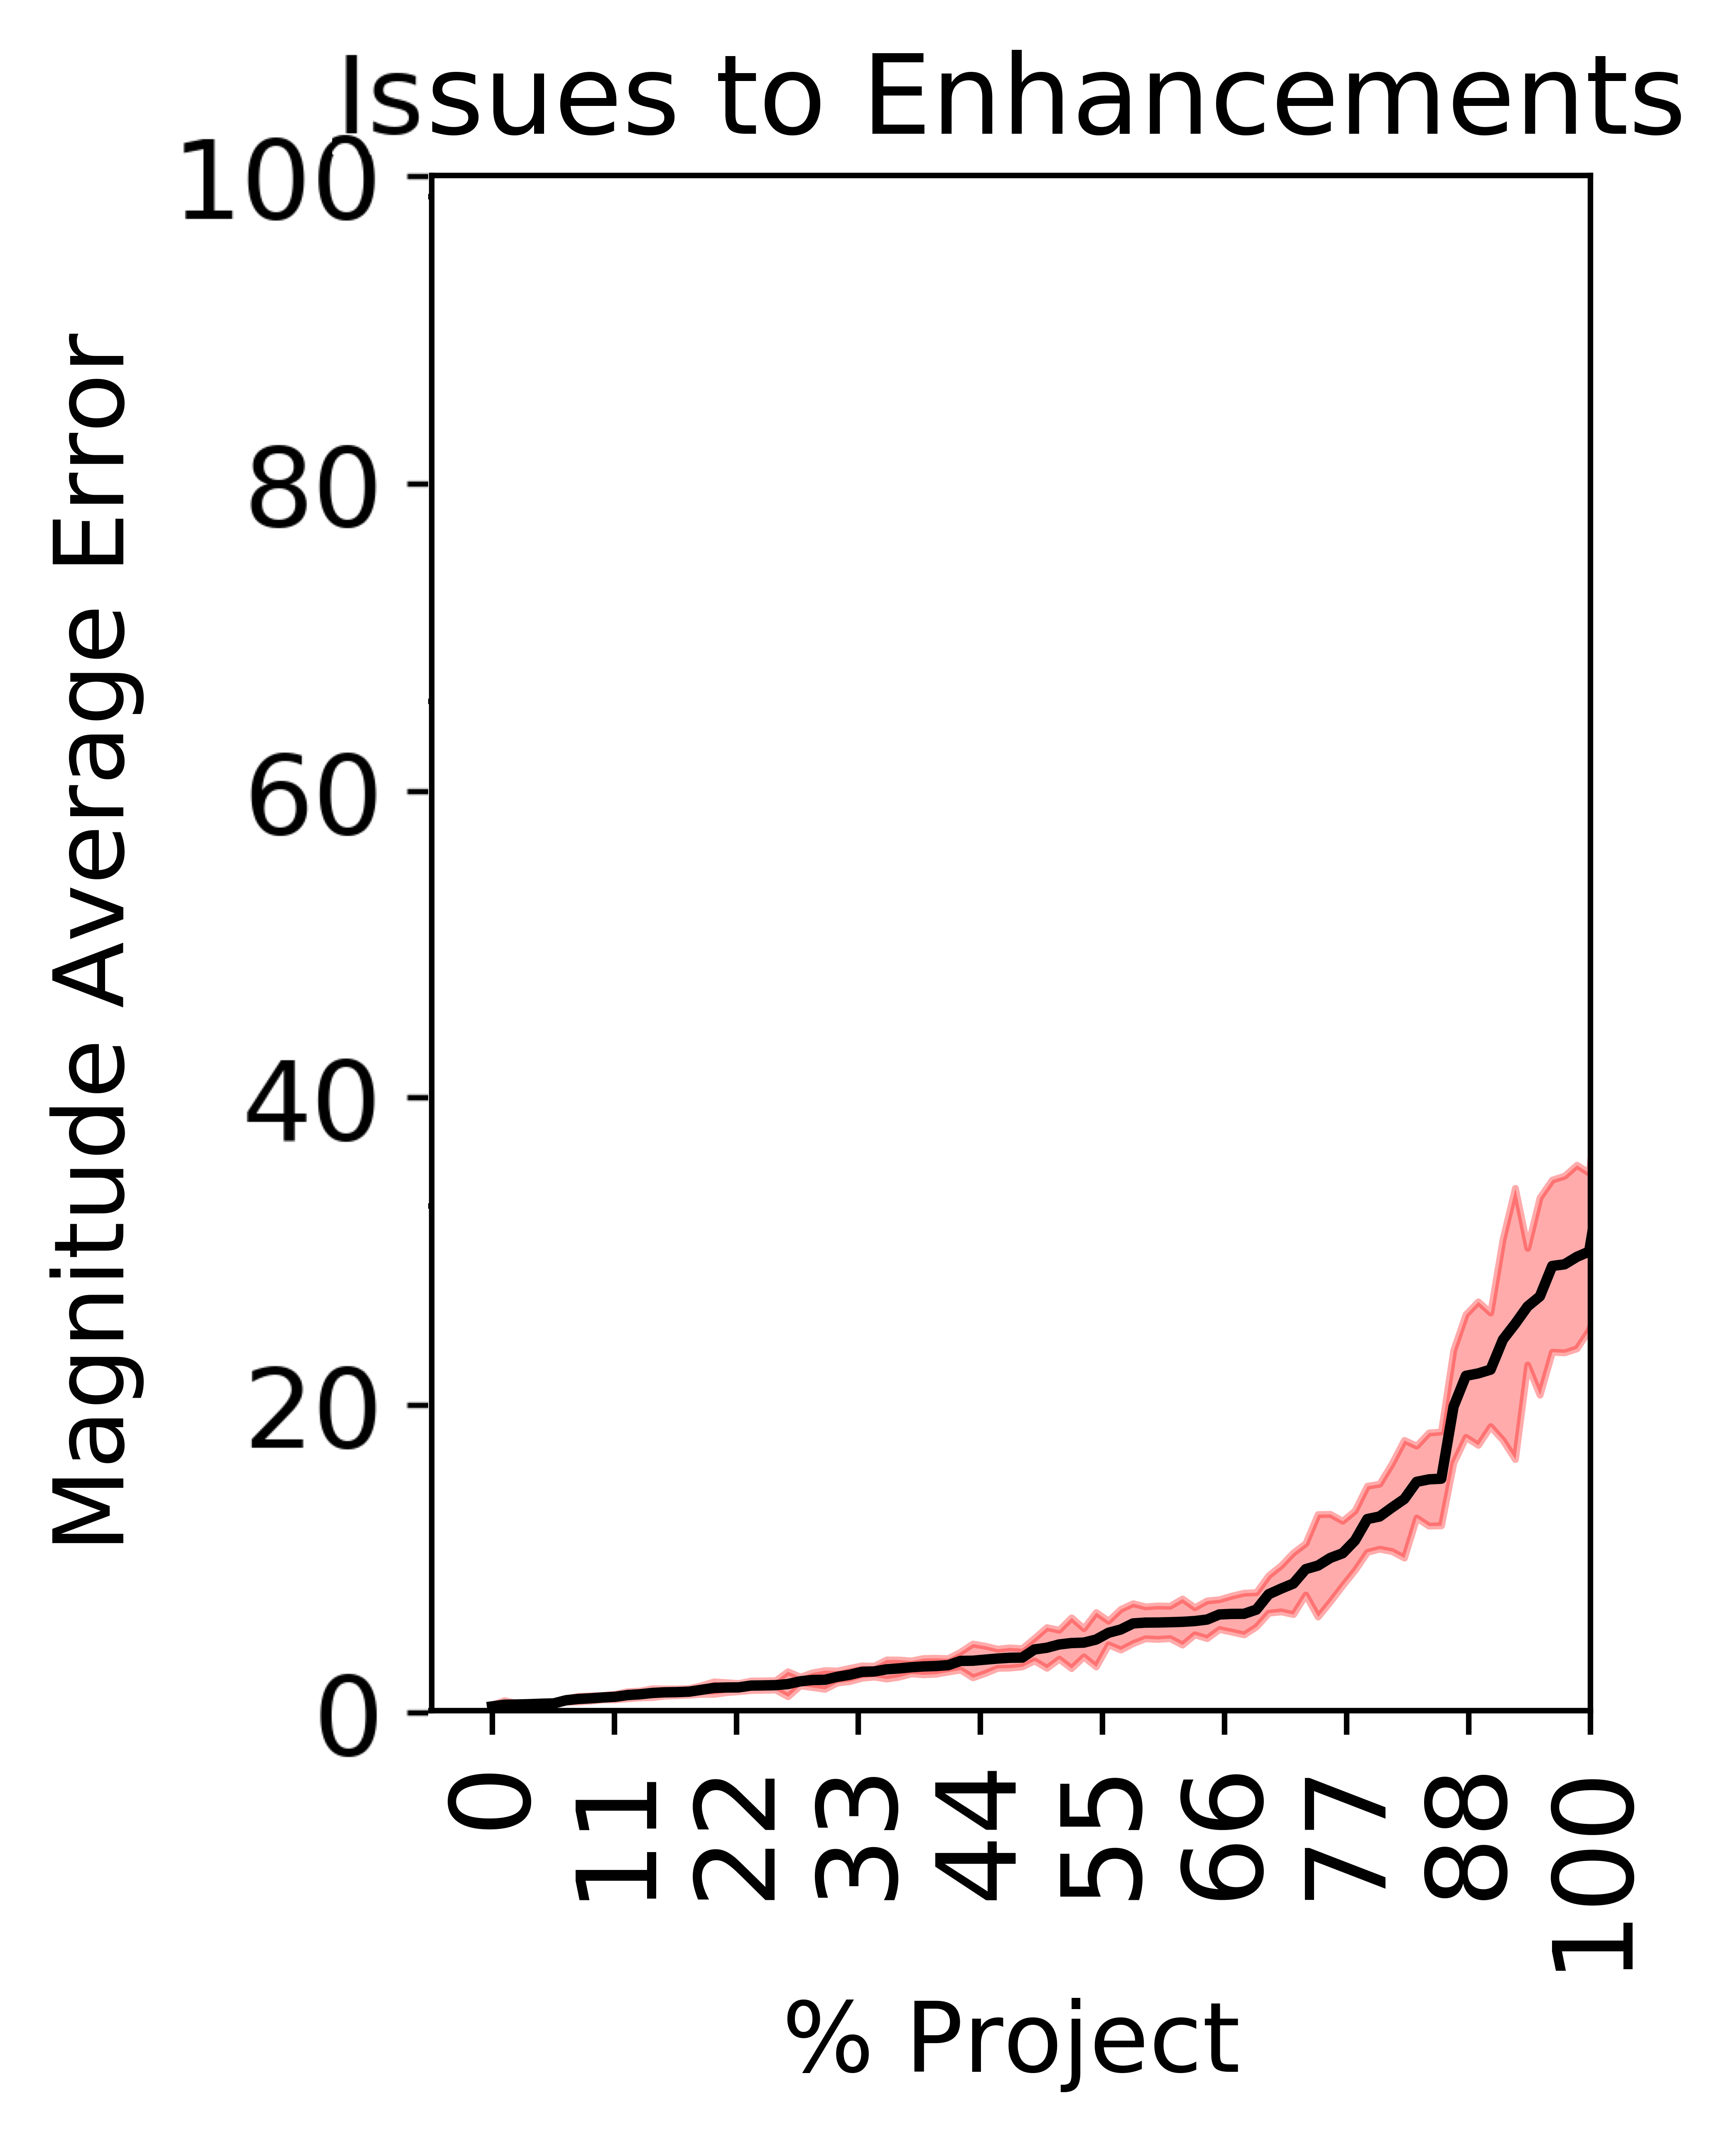
\includegraphics[width=0.334\linewidth]{images/RQ3/inhouse/enhancements/1.png}
		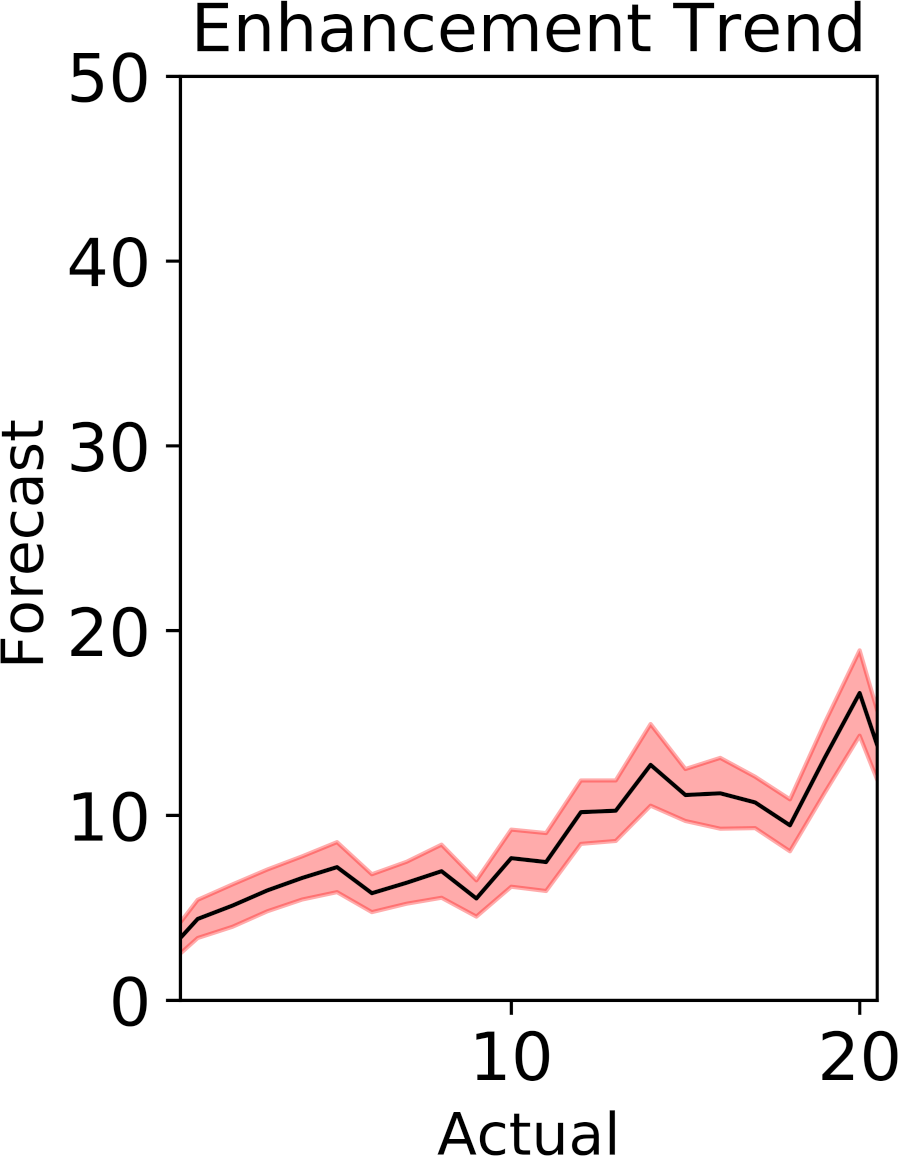
\includegraphics[width=0.32\linewidth]{images/RQ3/inhouse/enhancements/2.png}
	\end{subfigure}%
	\\[0.2cm]
	\textbf{Opensource}
	\\[0.1cm]
	\begin{subfigure}[t]{0.5\linewidth}
		\centering
		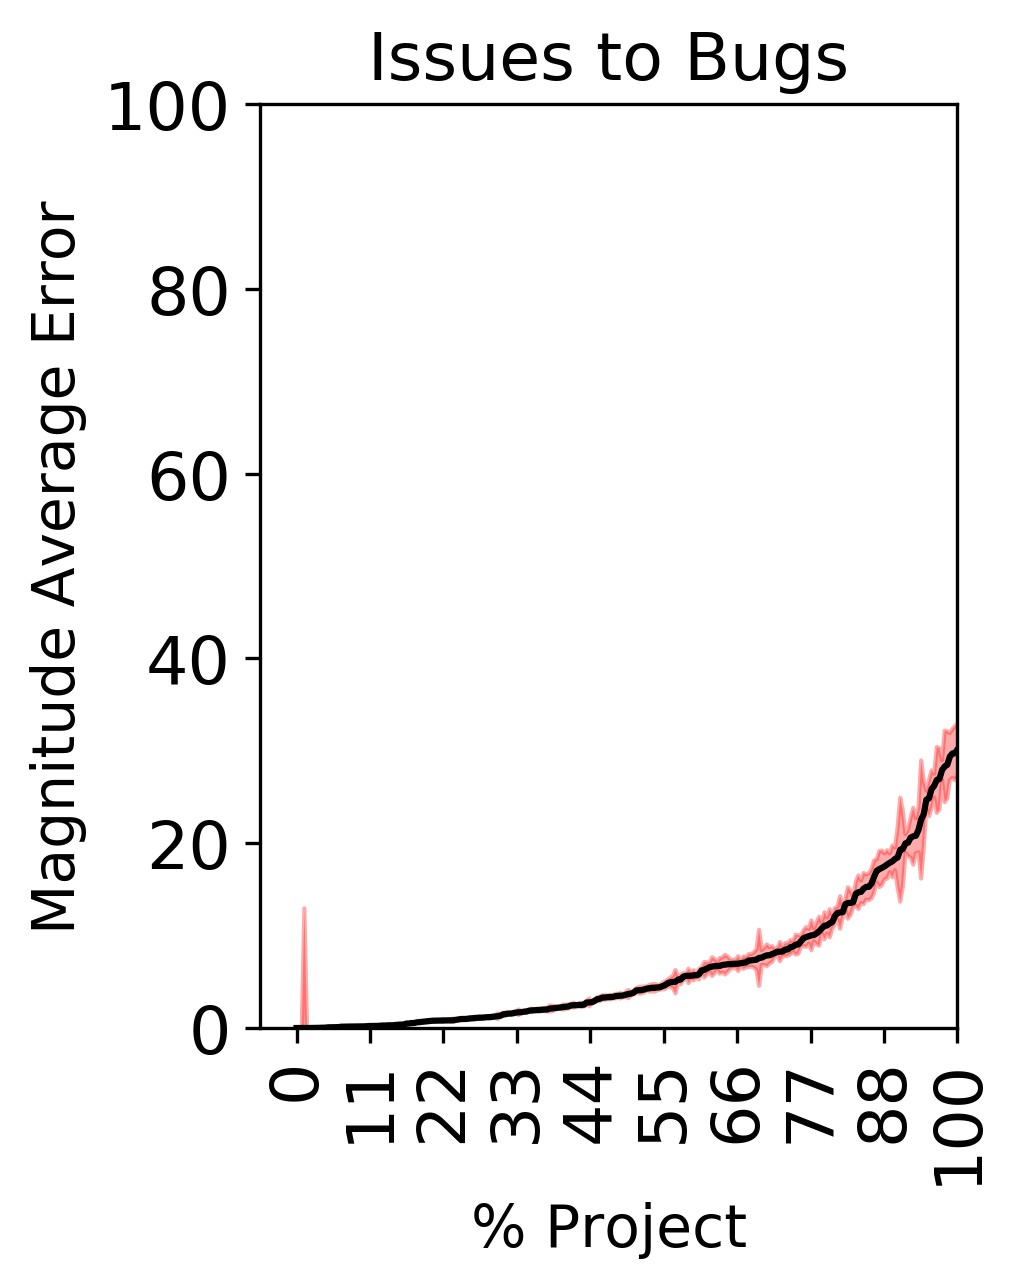
\includegraphics[width=0.335\linewidth]{images/RQ3/opensource/bugs/1.png}
		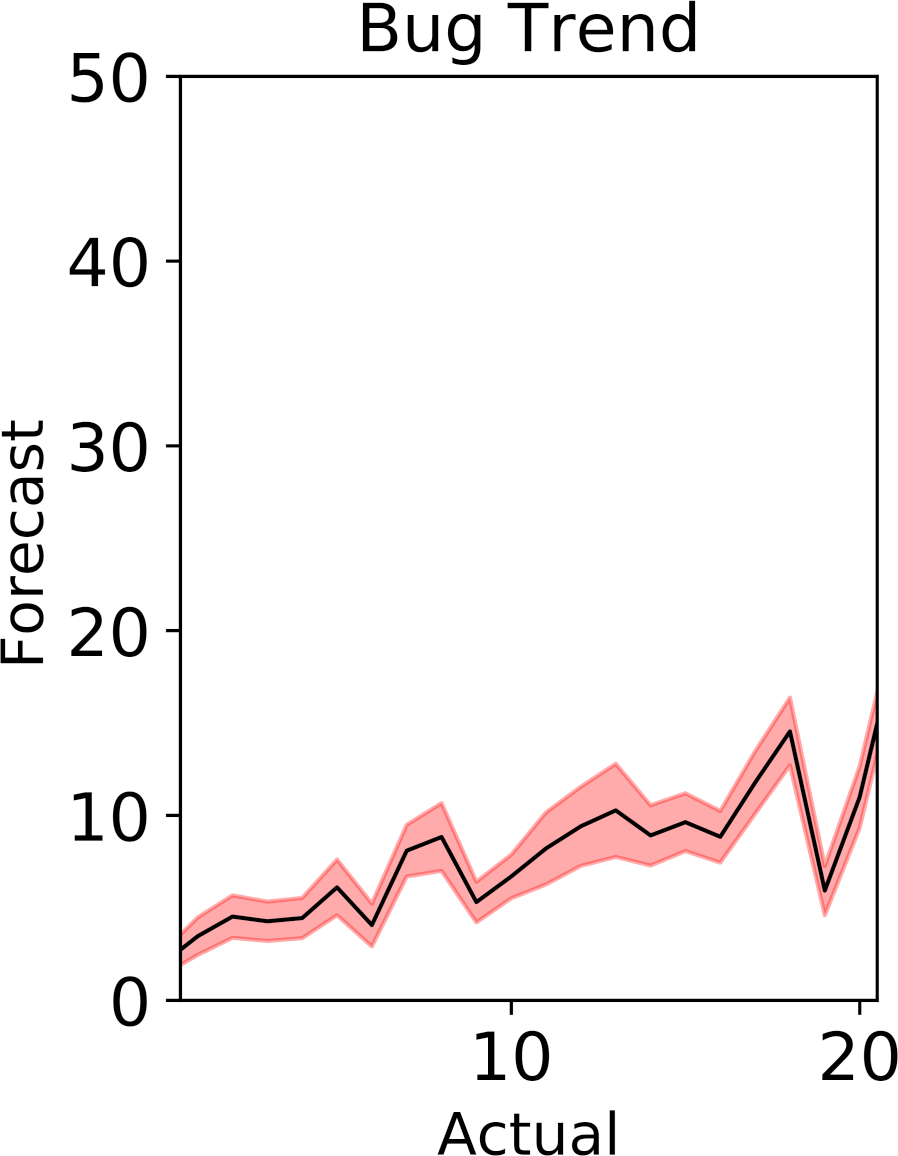
\includegraphics[width=0.33\linewidth]{images/RQ3/opensource/bugs/2.png}
	\end{subfigure}%
	%
	\centering
		\begin{subfigure}[t]{0.5\linewidth}
		\centering
		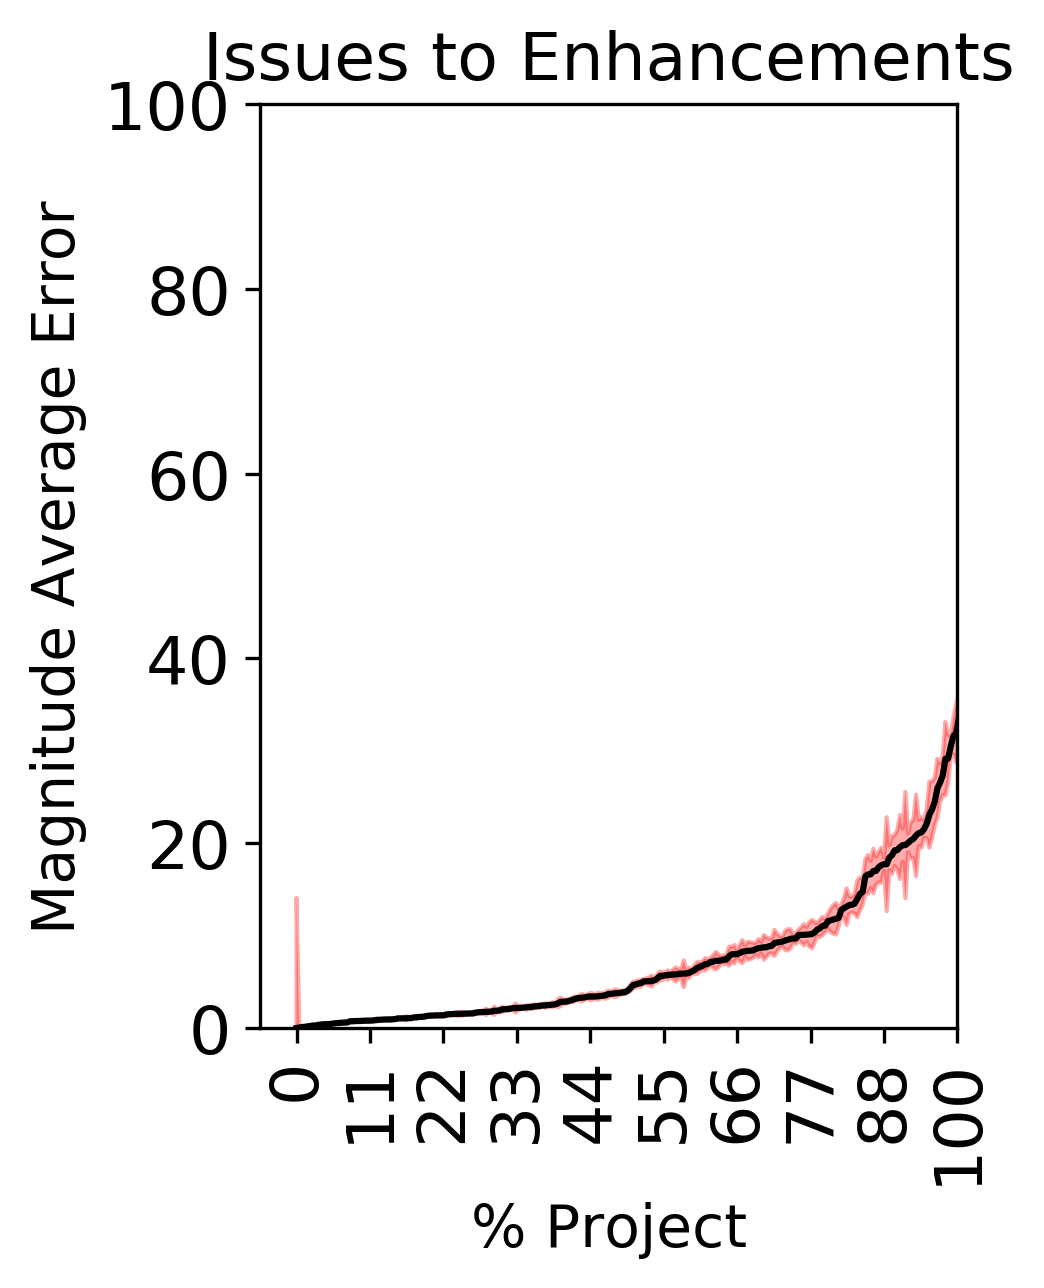
\includegraphics[width=0.334\linewidth]{images/RQ3/opensource/enhancements/1.png}
		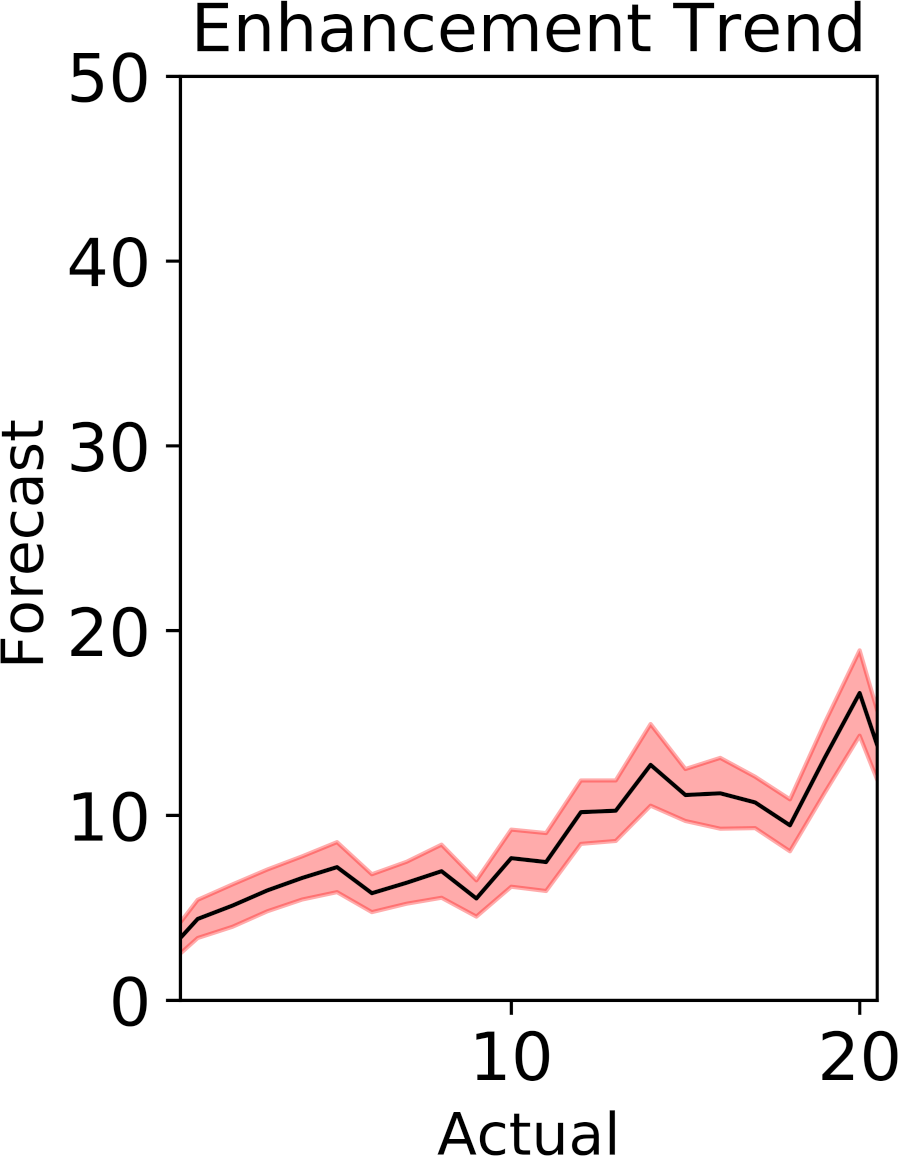
\includegraphics[width=0.32\linewidth]{images/RQ3/inhouse/enhancements/2.png}
	\end{subfigure}%
	\caption{This figure shows forecasts for future bugs and enhancements using ARIMA models constructed using past issue reports. For both proprietary and opensource projects, the magnitude of average error is very low (close to zero in several cases). Trend graphs show that an increase in actual bugs (or enhancements) leads to a corresponding increase in forecasts.}
	\label{fig:rq3}
\end{figure*}
